% !TeX spellcheck = en_US
% !TeX encoding = utf8
% !TeX program = pdflatex

% \pdfminorversion=4
\documentclass[	%10pt
				% ,handout
				% ,notes=show
				% ,draft
				]{beamer}


\usepackage[T1]{fontenc}
\usepackage{rubfonts2009}
\usepackage{import}
\usetheme[alternativetitlepage=normal]{Rub}
% \usetheme{Berlin}
\usepackage{bm}
% \usetheme{Warsaw}
% \usecolortheme{seahorse}
% \usecolortheme{rose}
% \usefonttheme[onlylarge]{structuresmallcapsserif}
% \usefonttheme[onlysmall]{structurebold}
\setbeamercovered{transparent}
\usepackage{pgfplots}
\usepackage{intcalc}
\usepackage{graphicx}
\usepackage{amsmath}
\usepackage{array}
\usepackage{amssymb}
\usepackage{pgfplotstable}
\usepackage{caption}
\usepackage[
%disable
]{todonotes}
\usepackage[final]{pdfpages}
\usepackage{etoolbox}
\usepackage[backend=bibtex,style=alphabetic]{biblatex}


%broken biblatex http://tex.stackexchange.com/questions/311426/bibliography-error-use-of-blxbblverbaddi-doesnt-match-its-definition-ve
\makeatletter
\def\blx@maxline{77}
\makeatother

\usepackage{multirow}
\captionsetup[figure]{name=}

% \setbeamercolor{title}{fg=red!80!black}


\usepackage[english]{babel}
\usepackage[utf8]{inputenc}
\usetikzlibrary{shapes, arrows.meta, positioning, decorations.pathmorphing, math, calc, fit, chains, matrix, decorations.pathreplacing, trees, backgrounds, tikzmark}
%\usetikzlibrary{, , , , , , , ., , , }
\usepackage{xcolor}
% \usepackage[table]{xcolor}
\PassOptionsToPackage{table}{xcolor}
% \usepackage{tabularx}
% \usepackage{mathptmx,amsmath}
\usepackage{graphicx}
\linespread{1.3} % increase baselineskip (spacing between lines)
\title{Design and Implementation of an LDPC-based FEC encoder/decoder suitable for Storage devices}
% \subtitle[]{}
\author[Henry Bathke]{Henry Bathke}
\institute[RUB-ESIT]{Ruhr University of Bochum \linebreak Chair for Embedded Systems for Information Technology}
\date{15. March 2018}
\usetikzlibrary{shapes, arrows.meta, positioning, decorations.pathmorphing, math, calc}
\setbeamercolor{framesubtitle}{fg=gelbgruen}

\pgfplotscreateplotcyclelist{hollow}{%
	mark=o,color=red,thick\\%
	mark=square,color=brown,thick\\%
	mark=x,color=green!50!black,thick\\%
	mark=triangle,color=blue,thick\\%
	mark=diamond,color=black,thick\\%
}

\bibliography{../database.bib}

\AtBeginSection[]
{
  \begin{frame}[noframenumbering]
    \tableofcontents[currentsection, currentsubsection]
    \frametitle{Outline}
  \end{frame}
}
\AtBeginSubsection[]
{
  \begin{frame}[noframenumbering]
    \frametitle{Outline}
    \tableofcontents[currentsection,currentsubsection]
  \end{frame}
}


\graphicspath{ {image/} }

\setbeamercovered{invisible}
%%%%%%%%%%%%%%%%%%%%%%%%%%%%%%%     Title Page     %%%%%%%%%%%%%%%%%%%%%%%%%%%%%%%%%%%
\pgfplotsset{compat=1.16}
\begin{document}
	
\begin{frame}[plain]
  \titlepage
\end{frame}

%%%%%%%%%%%%%%%%%%%%%%%%%%%%%%%     Outline     %%%%%%%%%%%%%%%%%%%%%%%%%%%%%%%%%%%
\begin{frame}
  \frametitle{Outline}
  % \tableofcontents[pausesections]
  % \tableofcontents[hideallsubsections]
  \tableofcontents
\end{frame}

%%%%%%%%%%%%%%%%%%%%%%%%%%%%%%%     Motivation     %%%%%%%%%%%%%%%%%%%%%%%%%%%%%%%%%%%
\section{Motivation}
\begin{frame}
	\frametitle{Motivation}
	\begin{itemize}
		\item Build a Hardware encoder and decoder suitable for storage devices
		\item Create a system for testing the encoder and decoder
	\end{itemize}

\end{frame}

%%%%%%%%%%%%%%%%%%%%%%%%%%%%%%%     Basics     %%%%%%%%%%%%%%%%%%%%%%%%%%%%%%%%%%%
\section{LDPC Codes}
\begin{frame}[fragile]
	\frametitle{Low Density Parity Check (LDPC) Codes}
	\begin{itemize}
		\item Multiple parity check equations
		\item Each bit is contained in multiple equations
		\item With these equations we can correct errors
		\item <2-> We construct the check matrix with the check equations
	\end{itemize}
	\visible<2->{
		\begin{align*}
			& \tikzmark{x1}x_1 \oplus \tikzmark{x2}x_3 \oplus \tikzmark{x3}x_4 \oplus \tikzmark{x4}x_7 = 0 \\
			\\
			\bm{H} = & \left[\begin{matrix}
				0 & \tikzmark{m1}1 & 0 & \tikzmark{m2}1 & \tikzmark{m3}1 & 0 & 0 & \tikzmark{m4}1 \\ 
				1 & 1 & 1 & 0 & 0 & 1 & 0 & 0 \\
				0 & 0 & 1 & 0 & 0 & 1 & 1 & 1 \\
				1 & 0 & 0 & 1 & 1 & 0 & 1 & 0
		\end{matrix}\right]	
		\end{align*}
		
		\begin{tikzpicture}[remember picture,overlay]
			%\draw[->] 
			\draw[->] ([shift={(1ex,-1ex)}]pic cs:x1) -- ([shift={(1pt,1em)}]pic cs:m1);
			\draw[->] ([shift={(1ex,-1ex)}]pic cs:x2) -- ([shift={(1pt,1em)}]pic cs:m2);
			\draw[->] ([shift={(1ex,-1ex)}]pic cs:x3) -- ([shift={(1pt,1em)}]pic cs:m3);
			\draw[->] ([shift={(1ex,-1ex)}]pic cs:x4) -- ([shift={(1pt,1em)}]pic cs:m4);
		\end{tikzpicture}
	}
\end{frame}

\begin{frame}
	\frametitle{Quasi Cyclic Low Density Parity Check (LDPC)}
	\begin{itemize}
		\item High complexity of LDPC codes
		\item Reduce complexity by adding structure to the PCM
		\item Split PCM into submatrices
		\item Only allow shifted version of a submatrix
	\end{itemize}
	\begin{equation*}
		\bm{B} = \left[\begin{matrix}
			-1 & 0 & 2 & -1\\
			0 & 1 & -1 & -1\\
			-1 & 1 & 0 & 2\\
		\end{matrix}\right]
	\end{equation*}
\end{frame}

%%%%%%%%%%%%%%%%%%%%%%%%%%%%%%%     Approach     %%%%%%%%%%%%%%%%%%%%%%%%%%%%%%%%%%%

\begin{frame}[fragile]
	\frametitle{Encoding}
	\begin{itemize}
		\item Is usually done with generator matrix
		\item The generator matrix is dense due to the inversion
		\item With long codes the dense matrix multiplication is large
		\item Use transforms on the PCM to convert it into a more desireable form
	\end{itemize}
	
\end{frame}

\begin{frame}[fragile]
	\frametitle{Encoding}
	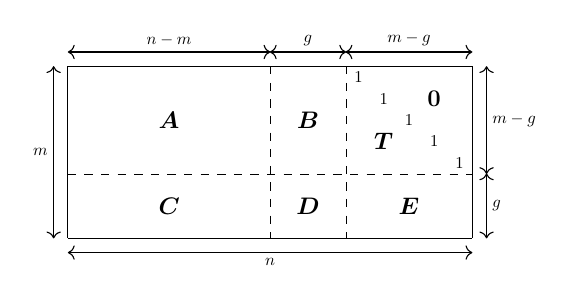
\begin{tikzpicture}[
		style1/.style={
				matrix of math nodes,
				every node/.append style={text width=#1,align=center,minimum height=3ex},
				nodes in empty cells,
			},
			scale=0.6,
			every node/.style={scale=0.6}
		]
		\matrix[style1=0.3cm] (1mat) {
			& & & & & & & & & & & & & & & \\
			& & & & & & & & & & & & & & & \\
			& & & & & & & & & & & & & & & \\
			& & & & & & & & & & & & & & & \\
			& & & & & & & & & & & & & & & \\
			& & & & & & & & & & & & & & & \\
			& & & & & & & & & & & & & & & \\
			& & & & & & & & & & & & & & & \\
		};
		\draw[dashed] (1mat-5-1.south west) -- (1mat-5-16.south east);
		\draw[dashed] (1mat-1-11.north east) -- (1mat-8-11.south east);
		\draw[dashed] (1mat-1-8.north east) -- (1mat-8-8.south east);

		\node [font=\Large] at ($(1mat-3-4)!0.5!(1mat-3-5)$) {$\bm{A}$};
		\node [font=\Large] at (1mat-3-10) {$\bm{B}$};

		\node [font=\Large] at (1mat-4-13) {$\bm{T}$};
		\node [font=\Large] at (1mat-2-15) {$\bm{0}$};

		\node [font=\Large] at ($(1mat-7-4)!0.5!(1mat-7-5)$) {$\bm{C}$};
		\node [font=\Large] at (1mat-7-10) {$\bm{D}$};
		\node [font=\Large] at (1mat-7-14) {$\bm{E}$};

		\node at (1mat-1-12) {1};
		\node at (1mat-2-13) {1};
		\node at (1mat-3-14) {1};
		\node at (1mat-4-15) {1};
		\node at (1mat-5-16) {1};
		
		\draw (1mat-1-1.north west) -- (1mat-8-1.south west);
		\draw (1mat-1-16.north east) -- (1mat-8-16.south east);
		\draw (1mat-1-1.north west) -- (1mat-1-16.north east);
		\draw (1mat-8-1.south west) -- (1mat-8-16.south east);

		\draw [<->] ([yshift=-3mm]1mat-8-1.south west) -- node[below] {$n$} ([yshift=-3mm]1mat-8-16.south east);
		\draw [<->] ([xshift=-3mm]1mat-1-1.north west) -- node[left] {$m$} ([xshift=-3mm]1mat-8-1.south west);

		\draw [<->] ([yshift=3mm]1mat-1-1.north west) -- node[above] {$n-m$} ([yshift=3mm]1mat-1-8.north east);
		\draw [<->] ([yshift=3mm]1mat-1-9.north west) -- node[above] {$g$} ([yshift=3mm]1mat-1-11.north east);
		\draw [<->] ([yshift=3mm]1mat-1-12.north west) -- node[above] {$m-g$} ([yshift=3mm]1mat-1-16.north east);

		\draw [<->] ([xshift=3mm]1mat-1-16.north east) -- node[right] {$m-g$} ([xshift=3mm]1mat-5-16.south east);
		\draw [<->] ([xshift=3mm]1mat-6-16.north east) -- node[right] {$g$} ([xshift=3mm]1mat-8-16.south east);
	\end{tikzpicture}
	\begin{itemize}
		\item Reach minimum gap $g$ by doing only row and column permutations
		\item Only need an inverted matrix of size $g \times g$
	\end{itemize}
\end{frame}

\begin{frame}
	\frametitle{Encoding}
	\begin{itemize}
		\item Only large sparse matrix multiplication and back substitution
		\item One small dense matrix multiplication
	\end{itemize}
	\begin{tabular}{l l}
		Operation & Type \\ \toprule
		$\bm{A}s^T$ & sparse multiplication \\
		$\bm{T}^{-1}\bm{A}s^T$ & sparse back substitution \\
		$-\bm{E}\bm{T}^{-1}\bm{A}s^T$ & sparse multiplication \\
		$\bm{C}s^T$ & sparse multiplication \\
		$\left(-\bm{E}\bm{T}^{-1}\bm{A}s^T\right) + \left(\bm{C}s^T\right)$ & vector addition \\
		$\bm{\phi}^{-1}\left(-\bm{E}\bm{T}^{-1}\bm{A}s^T + \bm{C}s^T\right)$ & dense $g\times g$ multiplication\\
	\end{tabular}
\end{frame}

\begin{frame}
	\frametitle{Encoding Hardware}
	\begin{itemize}
		\item Implemented as combinatorial logic
		\item Connects to the other modules with an axi stream bus
		\item Repacking is needed as bit counts dont evenly divide
	\end{itemize}
	\begin{itemize}
		\item make image with
		\item axi-stream to repack to encode to repack to axi-stream
	\end{itemize}
\end{frame}

\begin{frame}
	\frametitle{Decoding}
	\begin{itemize}
		\item I implemented a message passing decoder
		\item Messages are passed along the edges on the tanner graphicspath
		\item Computations are done on the nodes
	\end{itemize}
	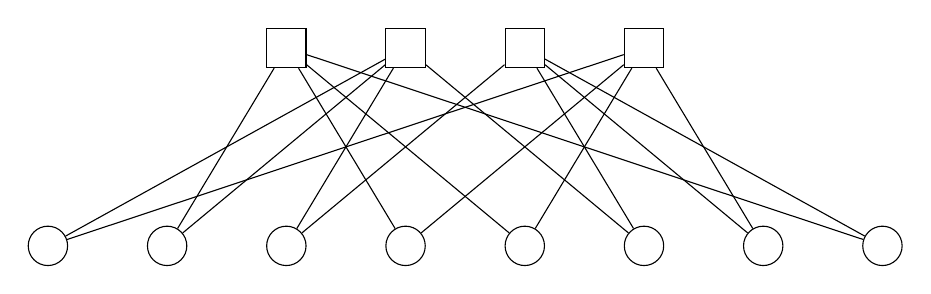
\begin{tikzpicture}[
		cnode/.style={draw,rectangle,node distance=1cm,align=center,minimum width=.5cm, minimum height=.5cm},
		vnode/.style={draw,circle,node distance=1cm,align=center,minimum width=.5cm, minimum height=.5cm}
	]
	\begin{scope}[start chain=going right, node distance=15mm]
		\node [vnode, on chain] (v0) {};
		\node [vnode, on chain] (v1) {};
		\node [vnode, on chain] (v2) {};
		\node [vnode, on chain] (v3) {};
		\node [vnode, on chain] (v4) {};
		\node [vnode, on chain] (v5) {};
		\node [vnode, on chain] (v6) {};
		\node [vnode, on chain] (v7) {};
	\end{scope}
	\begin{scope}[start chain=going right, node distance=15mm]
		\node [cnode, on chain, above=2cm of v2] (c0) {};
		\node [cnode, on chain] (c1) {};
		\node [cnode, on chain] (c2) {};
		\node [cnode, on chain] (c3) {};
	\end{scope}
	\draw (c0) -- (v1);
	\draw (c0) -- (v3);
	\draw (c0) -- (v4);	
	\draw (c0) -- (v7);
	\draw (c1) -- (v0);
	\draw (c1) -- (v1);
	\draw (c1) -- (v2);
	\draw (c1) -- (v5);
	\draw (c2) -- (v2);
	\draw (c2) -- (v5);
	\draw (c2) -- (v6);
	\draw (c2) -- (v7);
	\draw (c3) -- (v0);
	\draw (c3) -- (v3);
	\draw (c3) -- (v4);
	\draw (c3) -- (v6);
	\end{tikzpicture}
\end{frame}

\begin{frame}[fragile]
	\frametitle{Decoding}
	\begin{equation}
		r_{mn} = \left( \prod_{n' \in M(m)\\n}\sign(q_{n'm}) \right) \min_{n' \in vn\{m\}\\n}(\left|q_{n'm}\right|)
	\end{equation}
	\begin{itemize}
		\item 
	\end{itemize}
\end{frame}

%%%%%%%%%%%%%%%%%%%%%%%%%%%%%%%     Conclusion     %%%%%%%%%%%%%%%%%%%%%%%%%%%%%%%%%%%
\section{Conclusion}
\begin{frame}
	\frametitle{Conclusion}
	\begin{itemize}
		\item LDPC codes are usable with flash memory
		\item A latency vs. error correction capability trade off enables more control
		\item Overclocking directly improves user experience
	\end{itemize}
\end{frame}

\begin{frame}
	\frametitle{Questions?}
	\centering
	\Huge
	Questions?
\end{frame}

\begin{frame}[allowframebreaks]
	\frametitle{References}
	\linespread{1}
	\mode<handout>{
		\cite{CaiHaratschMutluMai2012}
		\cite{regulapati2015error}
		\cite{ZhaoVenkataramanZhang2014}
		\cite{ZhaoLiMaMicheloniZhang2014}
		\cite{zhao13}
	}
	\printbibliography
\end{frame}

\end{document}

